\chapter{DESENVOLVIMENTO}
\label{c.Desenvolvimento}

O desenvolvimento do projeto dividiu-se em quatro fases: a montagem do ambiente de testes de assinaturas construídas
a partir de regras do Yara; a obtenção das regras e construção de um índice de agrupamento das mesmas para agilizar a
execução das varreduras; obtenção e escolha de amostras de \textit{malware} para testagem; bateria de testes final e
análise de resultados. Complementarmente, foi desenvolvida a ideia de uma aplicação \textit{web} para análise
de \textit{malware} com base em regras de detecção do Yara.

\section{Obtenção das regras de detecção e das amostras de \textit{malware}}
\label{s.obtregras}

A primeira etapa da implementação computacional do projeto foi a construção de um índice de regras do Yara compilado a partir das
bases de assinaturas do ClamAV e de outros conjuntos avulsos e menores de assinaturas disponibilizados em repositórios de código
aberto; em paralelo, também construiu-se um conjunto de algumas amostras vivas e selecionadas de \textit{malware} para a testagem
do índice sobre arquivos infectados. Foram selecionadas apenas amostras de \textit{malware} `potencialmente inofensivo', como
\textit{trojans}, que dependem de um comando de execução disparado por um usuário descuidado, para que não houvesse risco de
propagação e infecção do próprio ambiente local e de redes com as quais o ambiente local se comunicasse. Por isso, com fins de
prevenção, optou-se pela não realização de testes em, por exemplo, \textit{worms}, que conseguem se propagar de maneira independente
pelos ambientes onde chegam.


\section{Testes iniciais com o ambiente de desenvolvimento}
\label{s.testesiniciais}

\section{Testagem completa e análise de resultados}
\label{s.testefull}

\section{Ideia de uma aplicação web do projeto desenvolvido}
\label{s.prototipo}

\begin{figure}
  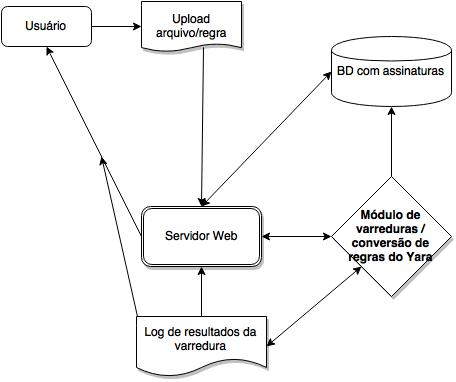
\includegraphics[scale=0.6]{figs/flux_prototipo}
  \centering
  \caption{Fluxograma de funcionamento da aplicação. Fonte: elaborada pelo autor.}
  \label{f.flux_prototipo}
\end{figure}
